\begin{figure}[htb]
  \centering
%segundo bloco de figuras
  \begin{tabular}{c c c c c }
    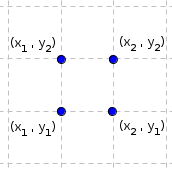
\includegraphics[width=3.5cm]{./img/dispositionFrameInGrid.png}    
    %& &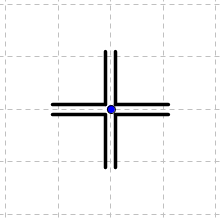
\includegraphics[width=4cm]{./img/truePieGrid.png} 
    & &
 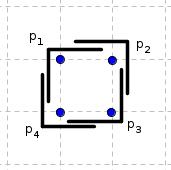
\includegraphics[width=3.5cm]{./img/frameInGrid.png} \\%[\abovecaptionskip]
    {\footnotesize (a) Pontos das coordenadas das dobras de uma moldura}  
    %& &  {\footnotesize (b) True pie} 
    & & {\footnotesize (c) Caminhos de uma moldura} %\label{fig:frame}
  \end{tabular}
  \caption{Representações $B_{1}$-EPG de um ciclo induzido de tamanho 4 por moldura} \label{fig:frameInGrid}
\end{figure} 